\documentclass[12pt,tikz]{standalone}
\usepackage[utf8]{inputenc}
\usepackage{amsmath}
\usepackage{pgfplots}
\usepackage{tikz}
\usetikzlibrary{calc}
\pagestyle{empty}

\begin{document}
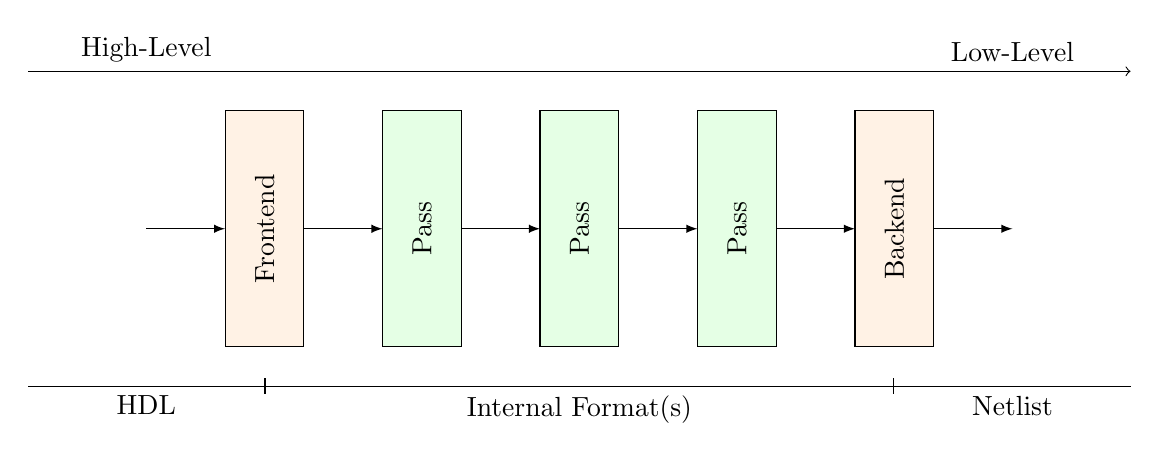
\begin{tikzpicture}
	\path (-1.5,3) coordinate (cursor);
	\draw[-latex] ($ (cursor) + (0,-1.5) $) -- ++(1,0);
	\draw[fill=orange!10] ($ (cursor) + (1,-3) $) rectangle node[rotate=90] {Frontend} ++(1,3) coordinate (cursor);
	\draw[-latex] ($ (cursor) + (0,-1.5) $) -- ++(1,0);
	\draw[fill=green!10] ($ (cursor) + (1,-3) $) rectangle node[rotate=90] {Pass} ++(1,3) coordinate (cursor);
	\draw[-latex] ($ (cursor) + (0,-1.5) $) -- ++(1,0);
	\draw[fill=green!10] ($ (cursor) + (1,-3) $) rectangle node[rotate=90] {Pass} ++(1,3) coordinate (cursor);
	\draw[-latex] ($ (cursor) + (0,-1.5) $) -- ++(1,0);
	\draw[fill=green!10] ($ (cursor) + (1,-3) $) rectangle node[rotate=90] {Pass} ++(1,3) coordinate (cursor);
	\draw[-latex] ($ (cursor) + (0,-1.5) $) -- ++(1,0);
	\draw[fill=orange!10] ($ (cursor) + (1,-3) $) rectangle node[rotate=90] {Backend} ++(1,3) coordinate (cursor);
	\draw[-latex] ($ (cursor) + (0,-1.5) $) -- ++(1,0);

	\path (-3,-0.5) coordinate (cursor);
	\draw (cursor) -- node[below] {HDL} ++(3,0) coordinate (cursor);
	\draw[|-|] (cursor) -- node[below] {Internal Format(s)} ++(8,0) coordinate (cursor);
	\draw (cursor) -- node[below] {Netlist} ++(3,0);

	\path (-3,3.5) coordinate (cursor);
	\draw[-] (cursor) -- node[above] {High-Level} ++(3,0) coordinate (cursor);
	\draw[-] (cursor) -- ++(8,0) coordinate (cursor);
	\draw[->] (cursor) -- node[above] {Low-Level} ++(3,0);

\end{tikzpicture}
\end{document}
